\section{Peer-to-Peer}
In a Peer-to-Peer system a peer acts as booth client and server at the same time meaning that it consumes content but also provides content for others. Unlike the traditional server-client model where the server acts as the single point of content distribution, Peer-to-Peer systems are not build on a centralised architecture so each peer can act autonomously and provide content to anyone else in the system.

As there is no central point there is also no single-point of failure and no single point as bottleneck. Thus a Peer-to-Peer can scale much better as described by \citet[\S1]{newscast-gossiping}:
\say{A well-designed peer-to-peer system can easily scale to millions of processes, each of which can join or leave whenever it pleases without seriously disrupting the system’s overall quality of service}. \citet[\S7.5.4]{tanenbaum_wetherall_2011} even go a step further and say that peer-to-peer system are \say{self-scaling}.
Due to its nature of design it is also hard to censorship or shut down a peer-to-peer system because there is no central server that someone can take control of. Also no one can harvest user data easily because the peers are connected autonomously with each other. Thus there is no central database that someone could attack or that can be used to monitor people in order to sell the data to 3rd parties.

According to \citet{tanenbaum_wetherall_2011} Peer-to-Peer systems have become popular in 1999 with the introduction of Napster, a Peer-to-Peer music streaming service. However, as it was mainly used to share copy-right infringed material, it was shutdown by government soon after. Shutting down the service was possible because Napster was not a fully decentralised Peer-to-Peer system. A central server was used as an index server to store the relation of content and who is hosting the content. Peers interested in content were querying the index server and got addresses as a result which were hosting the content matching to the search query. The content itself was exchanged in a peer-to-peer manner so the client opened a direct connection to the address to download the content. By shutting down the index server the peers could not locate any content anymore. 

The hybrid approach of Napster, using a index server was their solution of the complex problem of content discovery in a decentralised Peer-to-Peer network.

\subsection{Content Discovery}
Finding or publishing content in a peer-to-peer system is not a trivial task. In fact, depending on the structure of the Peer-to-Peer system, the size of the network and the chosen search strategy it might be impossible to find content, even though it might exist somewhere.

To discover content there are two typical scenarios:
\begin{itemize}
  \item Searching for content with a search query
  \item Finding content based on an address
\end{itemize}

\paragraph{Searching}
Based on the search query the system can be searched for content. When content exists the query returns a hit with the peers hosting the content. Peers are usually returned as addresses so a peer can connect to them.

In the example of Napster a user was publishing content by creating an entry on the index server with the actual content and its own address. Other peers were querying the index server with a search query. The index server looked up its own database for content matching the query. When content was available it returned the address of the host hosting the content. 

An approach that does not involve a central server is to use \textit{Flooding} to query all nodes in the network for content. One protocol that was using this approach is \textit{Gnutella} which has become popular soon after the shutdown of Napster.

The first version of the Gnutella Protocol was using \textit{Flooding} to disseminate a \textit{QUERY}-Packet through the network with the search query and a \gls{ttl}. When the client receiving the packet does not have content matching the query it forwards the query to all its neighbours as long as the \gls{ttl} allows re-broadcasting. A client that has content returns a query hit which is send back the same path as it came in \cite[\S4]{gnutella04}.

However as Gnutella became more and more popular scaling the system to support the growing amount of peers was crucial to keep the system alive. \say{LimeWire (a company promoting an enhanced Gnutella servent) suggested therefore the introduction of a two-level hierarchy: Ultrapeers (UPs) and Leaf
Nodes (LNs)} \cite[\S3.1]{gnutellaAnalysis}

By having a two-tier hierarchy the general \say{standby traffic} (traffic to maintain the overlay network) could be reduced.

Instead of flooding a \textit{QUERY}-Packet a \textit{Leaf Node} is now only send it to its \textit{Ultrapeer}. The Ultrapeers are connected with other Ultrapeers and have a distributed knowledge about content that is provided Leaf Nodes. When an Ultra Peer finds a Leaf Node that is providing content for the search query it is returning the address back to the originator of the query. The Gnutella protocol is further explained and evaluated by \citet{gnutellaAnalysis} but for the scope of this thesis not relevant.

\paragraph{Addressing}
In another scenario (cf. \vref{chap:IPFS}) the client already knows the content identifier and has to find the host which is providing the content.

In the server-client system this is done by addressing the server via its IP address and a path (\gls{url}) e.g. \textit{1.2.4.5/file/thesis.pdf}. The server is then looking up its file system and returns the content in case it is available.

The Peer-to-Peer system does not have a central file system and it would be infeasible to have one because that would mean that all the data from each peer would need to be replicated over all other peers.

So instead of using a \gls{url} a peer is addressing only the file but not a machine because it does not matter where the file is stored. This approach also makes it possible that the same content can be stored on multiple peers and the peer addressing the content gets it from a peer that works best for her (e.g. is the closest one).

To make the file addressable one option would be to use its file name. However the file name is just a meta information can be easily changed by the user so a file can exist on multiple machines with different file names. To generate a more unique identifier for a file, a better approach is to create a hash over the file content with a hash algorithm (e.g. SHA-256). As long as the file content does not change the hash will be always the same. The hash can be used as an address because it is unique for that specific file.

As the file is addressable by its content hash and as the same file can live on multiple peers other peer need to be able to find it in the network.

This is where the \gls{dht} comes into play.

\subsubsection{DHT}
\glsreset{dht}
As the name of the \gls{dht} indicates, it works like a hash table with a key–value pair but is distributed among multiple peers. By using a hash function an arbitrary value, that could be anything from an address to a file, is mapped to a key. The key space of the hash table is divided into buckets and distributed among the participants, each taking care of one bucket. This way, each participant is responsible for a bucket and does not need a global knowledge about all existing key–value pairs.

To assign buckets to peers, first of all they have to be uniquely identifiable as well. Thus each peer is assigned by an identifier from the same id-space as the keys from the hash table. This could be for example a hash over the \gls{ip} address of a peer with the same hash function that was used for the value hash e.g. SHA-256.

As the peer ids and the hash values are in the same id space the hash table can be partitioned into buckets by a distance function such as the value key has be the closest to a peer id and the value key has to be greater than the node key. Fulfilling both conditions means that a peer takes care of the key space from its own node id until its successor node id.

When a new node enters the network some of the key space has to be reorganised but not the whole key space. In fact, only the key space between the peer that is considered as a previous peer and the new peer has to be reorganised. This makes the \gls{dht} quite efficient as the remaining key space stays unaffected. 

A peer leaving the network is also removing all the content that it was hosting from th \gls{dht}. This is always a problem of Peer-to-Peer systems and the only way to prevent this is to replicate content over multiple peers. \citet[\S3]{chord} proposes some solutions how one could deal with such as \say{Coorparative Mirroring} or \say{Time-Shared Storage}.

Another condition to make the \gls{dht} work is that the participating peers form an overlay network so they can communicate with each other. This can be achieved for example with one of the routing protocols described in Mesh-Networking (\vref{chap:mesh-network}).

When a peer wants to enter content into the \gls{dht}, it generates the key for the content with the given hash function. The key is send together with the content to a known peer of the the \gls{dht} as \say{store-request}. When the peer is responsible for the key space of the given key it stores the key with the content otherwise it redirects the \say{store-request} to one of its known nodes where the peer id is closer to the key of the \say{store-request} of the overlay network. This step is repeated until the \say{store-request} reaches the peer responsible for the key space.

Looking up content in the \gls{dht} works in a similar way. A peer sends a \say{content-request} with a hash to a known entry point. When a peer is responsible for the key space or has stored the content by itself due to a previous request it returns the content. Otherwise it redirects the request to another peer where the peer id is closer to the hash of the \say{content-request}.

\subsubsection{\gls{dht} Implementations}
There are a several different DHT implementations out there like Chord \cite{chord}, Pastry \cite{pastry}, Tapestry \cite{tapestry} and Kademlia \cite{kademlia} to name just a few.
According to \citet[]{tanenbaum_wetherall_2011} \say{You will find it difficult to come up with a paper that is cited more than the seminal Chord paper}

\paragraph{Chord}
Chord uses consistent hashing which balances the load with a high probability due to design of consistent hashing. \citet{consistentHashing} explains Consistent Hashing as \say{a distributed hashing scheme that operates independently of the number of servers or objects in a distributed hash table by assigning them a position on an abstract circle, or hash ring. This allows servers and objects to scale without affecting the overall system.} \citet[\S4.2]{chord} point out a big advantage: \say{
Consistent hashing is designed to let nodes enter and leave the network with minimal disruption}
Peers are placed in an abstract circle with a size $\ m $ based on their hashed peer id where each peer is followed by a peer with a higher node id (successor). In a very basic implementation of Chord a peer only needs to know it successor peer. When a key id is queried each peer is passing it to its successor until it reaches the peer that is responsible of the key space. However, this is not not very efficient because in the worst case a query has to pass the whole circle until it finds its destination. To improve efficiency Chord introduces a finger table where each peer $\ n $ contains the address of the successor for each entry $\ i $ and $\ (n + 2^{i-1}) \mod 2^m $ where $\ m $ is the size of the circle and $\ 1 \leq i \leq m$. Through the finger table a peer can efficiently route a query request to its destination by using a known peer that is closer to the queried key. \citet[\S4.3]{chord} describe the process in their paper the following: \say{If $\ n $ can find a node whose ID is closer than its own to $\ k $, that node will know more about the identifier circle in the region of$\ k $ than $\ n $ does. Thus $\ n $ searches its finger table for the node $\ j $ whose ID most immediately precedes $\ k $, and asks $\ j $ for the node it knows whose ID is closest to $\ k $. By repeating this process, $\ n $ learns about nodes with IDs closer and closer to $\ k $}.

\paragraph{Kademlia}
Kademlia claims to be better than Chord by using a novel \gls{xor} metric which enables them to have a symmetry between keys and node ids \cite[\S1]{kademlia}. They also claim to be better than other algorithms like Pastry in terms of routing, by having one single routing algorithm to locate a peer for a key, while \say{other systems use one algorithm to get
near the target ID and another for the last few hops}\cite[\S1]{kademlia}

The \gls{xor} metric is used to determine a distance from on key to another. As both the node ids and the keys of the \gls{dht} are in the same key space this is used to find a node that is closer to the given key. Unlike other distances e.g. euclidian distance it is always unique.
Given the nodes with $\ id = 5 $ in the decimal space, which is  $\ 0101_{b} $ in the binary space, $\ id = 4 = 0100_{b} $ and $\ id = 3 = 0011_{b} $ the euclidean distance $\ d_{euclidean}(5,4) $ and $\ d_{euclidean}(3,4) $ would be the same while the xor distance differs.
\begin{equation}
\begin{aligned}  
    d_ {euclidean} = & | 5-4 | = 1\\
    d_ {euclidean} = & | 3-4 | = 1\\
    d_ {\gls{xor}} = & 0101_{b} \oplus 0100_{b} = 0001_{b} = 1\\
    d_ {\gls{xor}} = & 0011_{b} \oplus 0100_{b} = 0111_{b} = 7\\
  \end{aligned}  
\end{equation}
The \gls{xor} metric is also symmetric $\ d_{\gls{xor}}(a,b) = d_{\gls{xor}}(b,a) $, the distance to itself is zero $\ d_{\gls{xor}}(a,a) = 0 $ and it full fills the triangle inequality $\ d_{\gls{xor}}(a,b) \oplus d_{\gls{xor}}(b,c) = d_{\gls{xor}}(a,c) $ \cite{kademlia}[\S2.1].

By using a binary format for the ids, Kademlia creates a virtual binary tree for each node where each other node is treated as a leaf node. Thereby the binary tree is divided into subtrees where \say{the highest subtree consists of the half of the binary tree not containing the node. The next subtree consists of the half of the remaining tree not containing the node, and so forth} \cite[\S2]{kademlia}.
\vref{fig:kad-binary-tree} shows a sample binary tree for the black node with the id 0011 with its subtrees that are circled.

\begin{figure}
\centering
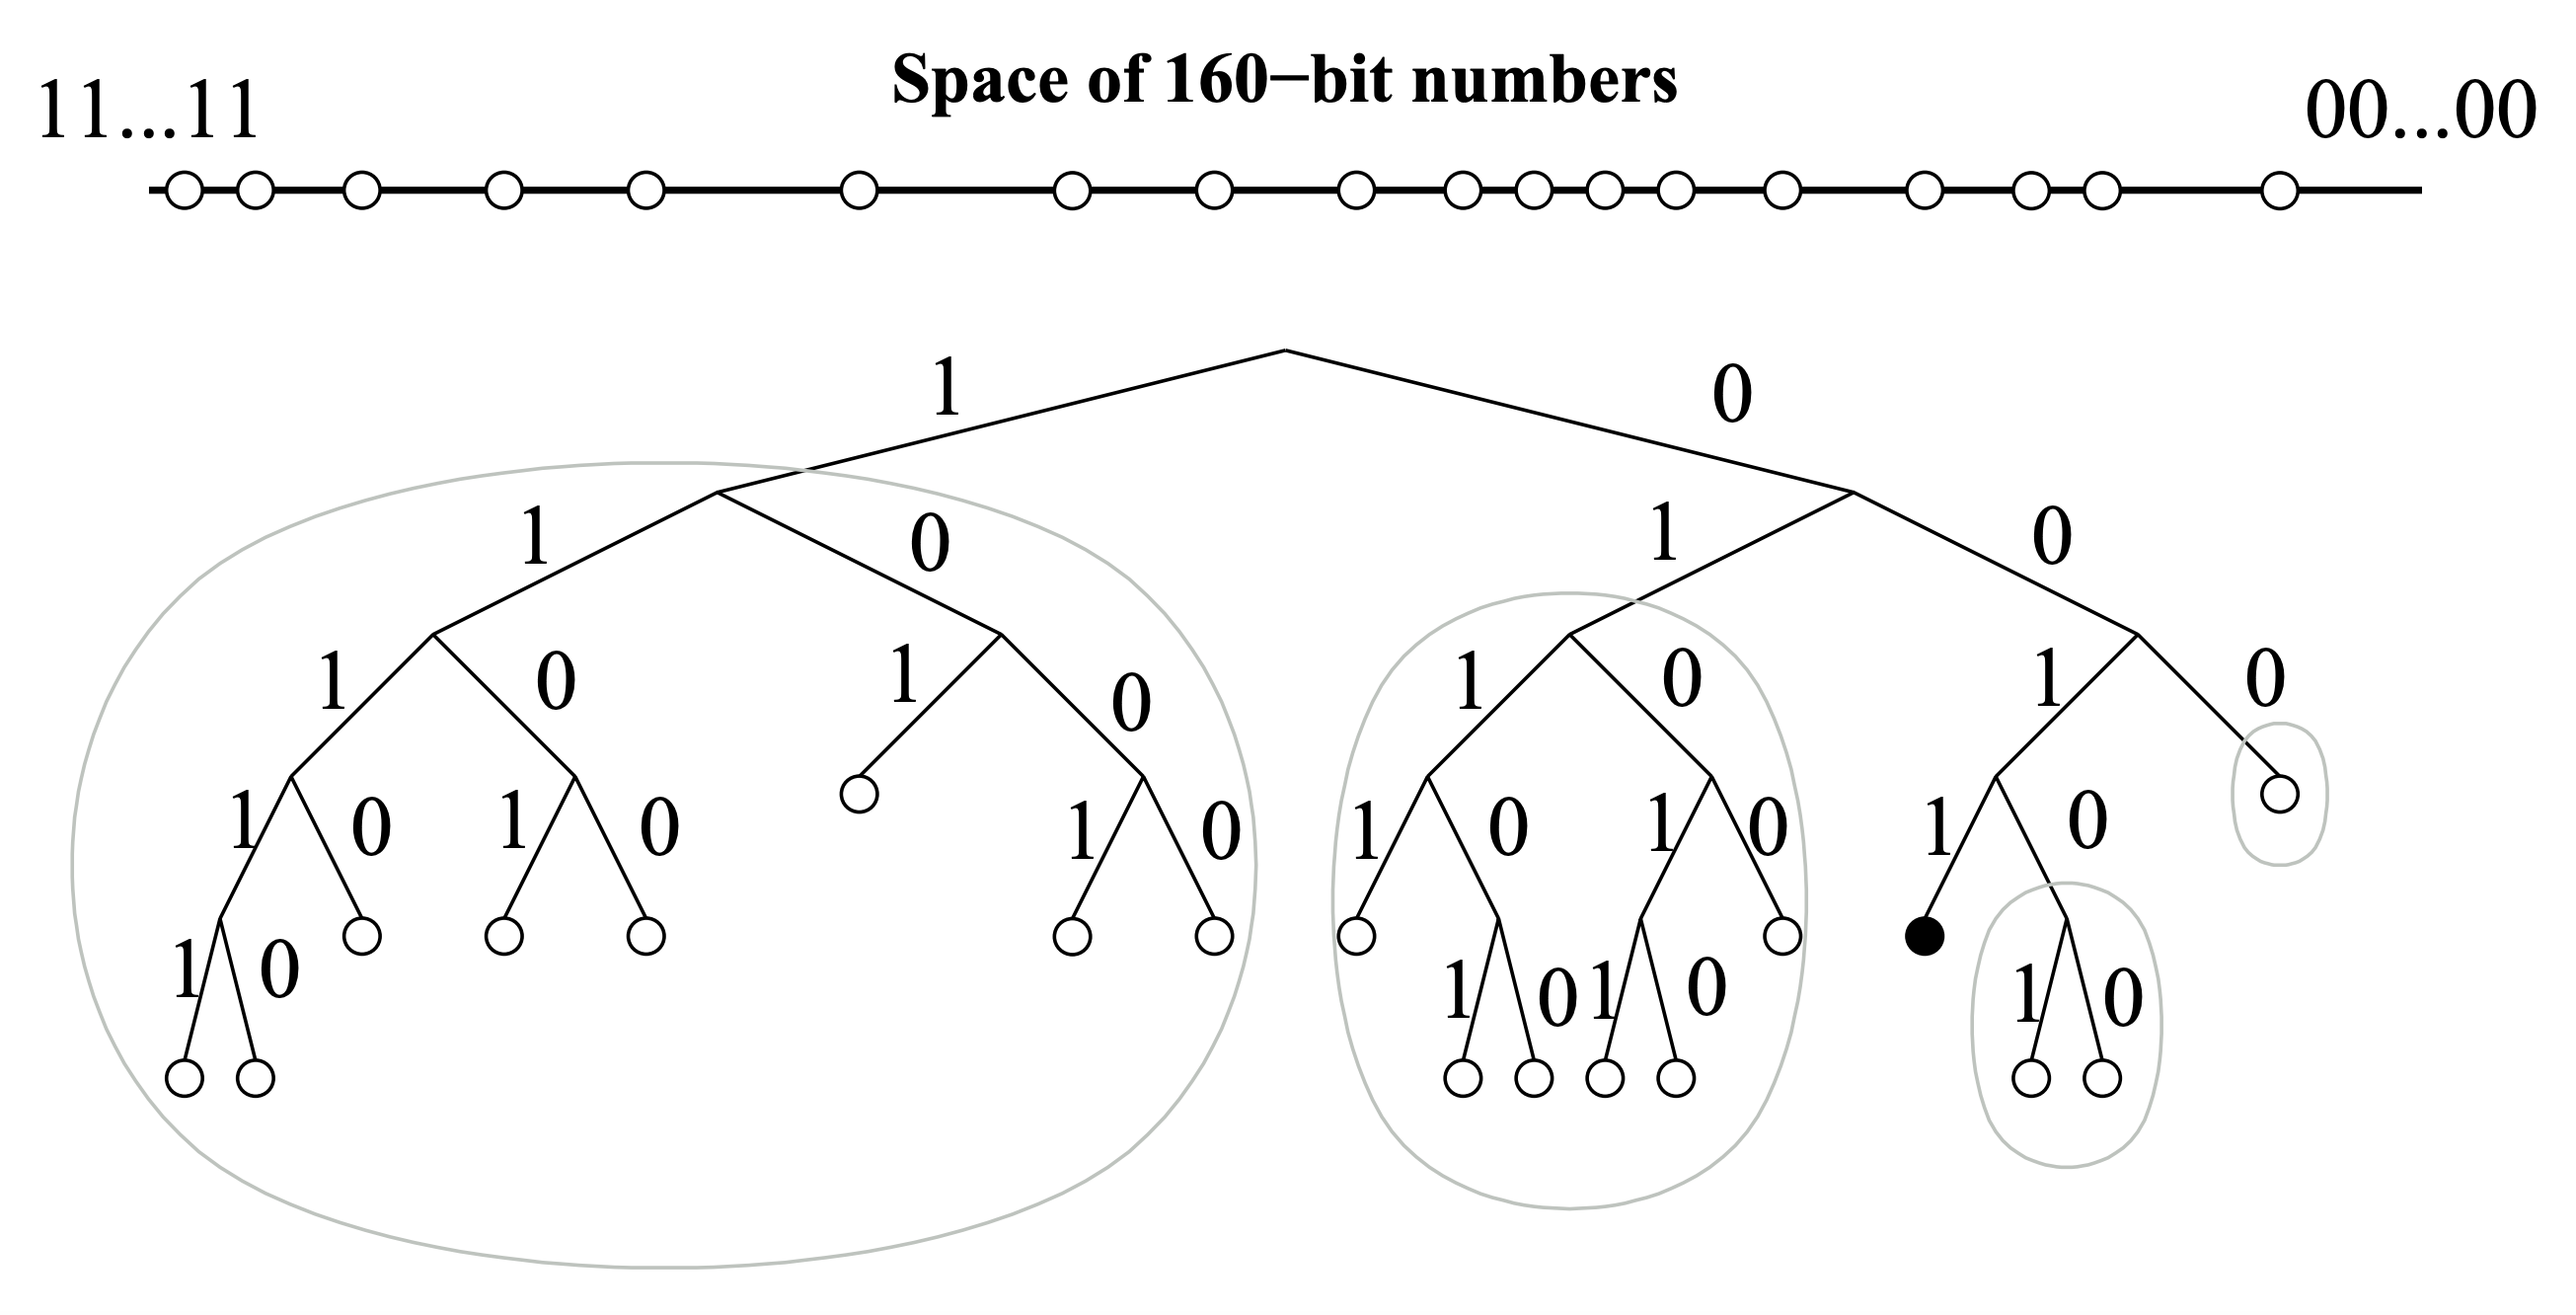
\includegraphics[width=1\textwidth]{graphics/kademlia-binary-tree.png}
\caption{Kademlia binary tree from \cite[\S2]{kademlia}}
\label{fig:kad-binary-tree}
\end{figure}

A node is discovering other nodes over time during message exchanges. Discovered nodes are stored in \say{k-buckets}. Each \say{k-bucket} represents a subtree of the node's virtual binary tree and can have $\ k $ entries. The \say{k-buckets} prevent that the routing table of a node grows to big and also prevents that only close by nodes are stored. By having the $\ k $ limitation which Kademlia sets to $\ 20 $ maximum 20 discovered node can be stored in each bucket. 
Each entry of the bucket has a \textit{last-seen} property that is updated whenever a message of the node is received. The bucket is sorted by \textit{last-seen}. When a new node is discovered but the bucket is already full Kademlia puts older entries in favour as long as they are alive. To check the liveliness it pings the least recently seen entry in the table. When the node responds the new discovered node is discarded. However, when the pinged node does not respond it is removed from the bucket and replaced with the newly discovered node. \citet[\S2.2]{kademlia} argues this with \say{The longer a node has been up, the more likely it is to remain up another hour.}

The design of the protocol ensures that each node knows at least one other node of each subtree and therefore a node can find any other node by its id. To find a \textit{Node X} a \textit{Node A} sends a \textit{FIND\_NODE} request to a node of its buckets that is closest to \textit{Node X} in terms of the \gls{xor} distance. This \textit{Node B} will then return a \textit{Node C} that is closer to \textit{Node X}. \textit{Node A} will then ask \textit{Node C} for the closest node it knows for the \textit{Node X}. This step is repeated until \textit{Node A} finds \textit{Node X}. To speed up the process not only one node is asked but multiple nodes that are the closest are asked in parallel. Those nodes also return the closest nodes they know.

Keys are also looked up similar like nodes. A key is stored at a node that is closest to the node id by the \gls{xor} distance. When a node wants to publish a key it sends a \textit{STORE} request to known nodes that are the closest to the id.
To lookup a key a node sends a \textit{FIND\_VALUE} request to the closest nodes. The process works like finding a node but it terminates as soon as one node returns the stored key.

\subsection{Peer Discovery}
To enter a Peer-to-Peer system there has to be an entry point where new peers can join. 
\citet{p2p-bootstrapping} describe this procedure as \say{P2P bootstrapping}. 
They also give three definitions for the term \say{P2P Bootstrapping}:
\begin{quote}
    \begin{itemize}
        \item Starting a new P2P network (freshly designed protocol)
        \item Once a P2P network is running, any new peer that joins must be integrated into the network
        \item Before a new peer can be integrated into an existing network, the new peer must somehow obtain contact information to at least one node in the existing P2P network
    \end{itemize}
\end{quote} \citet[p.3]{p2p-bootstrapping}

One approach for the boarding process is a central server that provides a list of addresses where a client can enter. In early days of Gnutella a user could enter the network by getting some addresses from a website and pasting them into the Gnutella client \cite{gnutellaAnalysis}[\S3.2]. However, due to Peer Churn it was hard to keep the list of addresses up to date, which resulted in a lot of addresses of peers that were not in the network anymore. In a later version Gnutella tried to solve the problem by providing \say{Gnutella Web Cache} Servers which were mainting a list of active peers. A client could conneet to a \say{Gnutella We Cache} server to obtain a list of active peers to enter the network. Problems that are arising of having a server is that the server is a single point of failure, may no

\subsection{Peer-to-Peer Issues}
- Peer Churn -> unstable network
- Leechers
- 
